%%%%%%%%%%%%%%%%%%%%%%%%%%%%%%%%%%%%%%%%%%%%%%%%%%%%%%%%%%%%%%%%%%%%%%%%%%%%%%%%
% Template for USENIX papers.
%
% History:
%
% - TEMPLATE for Usenix papers, specifically to meet requirements of
%   USENIX '05. originally a template for producing IEEE-format
%   articles using LaTeX. written by Matthew Ward, CS Department,
%   Worcester Polytechnic Institute. adapted by David Beazley for his
%   excellent SWIG paper in Proceedings, Tcl 96. turned into a
%   smartass generic template by De Clarke, with thanks to both the
%   above pioneers. Use at your own risk. Complaints to /dev/null.
%   Make it two column with no page numbering, default is 10 point.
%
% - Munged by Fred Douglis <douglis@research.att.com> 10/97 to
%   separate the .sty file from the LaTeX source template, so that
%   people can more easily include the .sty file into an existing
%   document. Also changed to more closely follow the style guidelines
%   as represented by the Word sample file.
%
% - Note that since 2010, USENIX does not require endnotes. If you
%   want foot of page notes, don't include the endnotes package in the
%   usepackage command, below.
% - This version uses the latex2e styles, not the very ancient 2.09
%   stuff.
%
% - Updated July 2018: Text block size changed from 6.5" to 7"
%
% - Updated Dec 2018 for ATC'19:
%
%   * Revised text to pass HotCRP's auto-formatting check, with
%     hotcrp.settings.submission_form.body_font_size=10pt, and
%     hotcrp.settings.submission_form.line_height=12pt
%
%   * Switched from \endnote-s to \footnote-s to match Usenix's policy.
%
%   * \section* => \begin{abstract} ... \end{abstract}
%
%   * Make template self-contained in terms of bibtex entires, to allow
%     this file to be compiled. (And changing refs style to 'plain'.)
%
%   * Make template self-contained in terms of figures, to
%     allow this file to be compiled. 
%
%   * Added packages for hyperref, embedding fonts, and improving
%     appearance.
%   
%   * Removed outdated text.
%
%%%%%%%%%%%%%%%%%%%%%%%%%%%%%%%%%%%%%%%%%%%%%%%%%%%%%%%%%%%%%%%%%%%%%%%%%%%%%%%%

\documentclass[letterpaper,twocolumn,10pt]{article}
\usepackage{usenix2019_v3}

% to be able to draw some self-contained figs
\usepackage{tikz}
\usetikzlibrary{crypto.symbols}
\tikzset{shadows=no} 
\usetikzlibrary{positioning}
\usetikzlibrary{shapes}
\usepackage{rotating} 
\usepackage{amsmath}
\usepackage{algorithm}% http://ctan.org/pkg/algorithms
\usepackage{algpseudocode}% http://ctan.org/pkg/algorithmicx



% inlined bib file
\usepackage{filecontents}
\newtheorem{theorem}{Theorem}

%-------------------------------------------------------------------------------
\begin{filecontents}{\jobname.bib}
%-------------------------------------------------------------------------------
  % Collision Research
  @article{klima2006tunnels,
  title={Tunnels in Hash Functions: MD5 Collisions Within a Minute.},
  author={Klima, Vlastimil},
  journal={IACR Cryptology ePrint Archive},
  volume={2006},
  pages={105},
  year={2006}
  note =         {\url{https://pdfs.semanticscholar.org/303a/13faac4a76c2e249fcd9587257f276da1a02.pdf}}
}
@inproceedings{wang2005break,
  title={How to break MD5 and other hash functions},
  author={Wang, Xiaoyun and Yu, Hongbo},
  booktitle={Annual international conference on the theory and applications of cryptographic techniques},
  pages={19--35},
  year={2005},
  organization={Springer}
  note =         {\url{https://link.springer.com/content/pdf/10.1007/11426639_2.pdf}}
}
@article{liang2007improved,
  title={Improved collision attack on hash function MD5},
  author={Liang, Jie and Lai, Xue-Jia},
  journal={Journal of Computer Science and Technology},
  volume={22},
  number={1},
  pages={79--87},
  year={2007},
  publisher={Springer}
  note =         {\url{http://citeseerx.ist.psu.edu/viewdoc/download?doi=10.1.1.81.8251&rep=rep1&type=pdf}}
}
@inproceedings{stevens2017first,
  title={The first collision for full SHA-1},
  author={Stevens, Marc and Bursztein, Elie and Karpman, Pierre and Albertini, Ange and Markov, Yarik},
  booktitle={Annual International Cryptology Conference},
  pages={570--596},
  year={2017},
  organization={Springer}
  note =         {\url{https://eprint.iacr.org/2017/190.pdf}}
}
@article{klima2005finding,
  title={Finding MD5 Collisions on a Notebook PC Using Multi-message Modifications.},
  author={Klima, Vlastimil},
  journal={IACR Cryptology ePrint Archive},
  volume={2005},
  pages={102},
  year={2005}
  note =         {\url{https://eprint.iacr.org/2005/102.pdff}}
}
@incollection{sasaki2006construct,
  title={How to construct sufficient conditions for hash functions},
  author={Sasaki, Yu and Naito, Yusuke and Yajima, Jun and Shimoyama, Takeshi and Kunihiro, Noboru and Ohta, Kazuo},
  booktitle={Progress in Cryptology-VIETCRYPT 2006},
  pages={243--259},
  year={2006},
  publisher={Springer}
  note = {\url{https://www.researchgate.net/profile/Sangjin_Lee6/publication/221462213_Improved_Fast_Correlation_Attack_on_the_Shrinking_and_Self-shrinking_Generators/links/02e7e52b36d7583923000000.pdf#page=252}}
}
@inproceedings{mironov2006applications,
  title={Applications of SAT solvers to cryptanalysis of hash functions},
  author={Mironov, Ilya and Zhang, Lintao},
  booktitle={International Conference on Theory and Applications of Satisfiability Testing},
  pages={102--115},
  year={2006},
  organization={Springer}
  note = {\url{https://eprint.iacr.org/2006/254.pdf}}
}
@article{bruce2004,
  title={Cryptanalysis of MD5 and SHA: Time for a New Standard},
  author={Schneier, Bruce},
  year={2004},
  publisher={Schneier on Security}
  note =         {\url{https://www.schneier.com/essays/archives/2004/08/cryptanalysis_of_md5.html}}
}
@article{merkle1979secrecy,
  title={Secrecy, authentication, and public key systems},
  author={Merkle, Ralph},
  journal={Ph. D. Thesis, Stanford University},
  year={1979}
  note =         {\url{http://www.merkle.com/papers/Thesis1979.pdf}}
}

@article{kurakin2016adversarial,
  title={Adversarial machine learning at scale},
  author={Kurakin, Alexey and Goodfellow, Ian and Bengio, Samy},
  journal={arXiv preprint arXiv:1611.01236},
  year={2016}
}

\end{filecontents}

%-------------------------------------------------------------------------------
\begin{document}
%-------------------------------------------------------------------------------

%don't want date printed
\date{}

% make title bold and 14 pt font (Latex default is non-bold, 16 pt)
\title{\Large \bf Blackbox Adversarial Learning on Hash Functions}

%for single author (just remove % characters)
\author{
{\rm Anirban Gangopadhyay}\\
Palantir Technologies
\and
{\rm Joshua Zweig}\\
Palantir Technologies
% copy the following lines to add more authors
% \and
% {\rm Name}\\
%Name Institution
} % end author

\maketitle

%-------------------------------------------------------------------------------
\begin{abstract}
%-------------------------------------------------------------------------------
We present a novel machine learning framework which we apply here to uncover weaknesses in hash functions. Our framework extends the definition of adversarial learning to the domain of cryptographic systems. In this paper, we uncover weaknesses in Merkle{\textendash}Damg\r{a}rd structured hash functions, which include MD5, SHA-1 and SHA-2 and are critical components of cryptographic systems such as key exchange, digital signatures, and password and file verification. Most attacks against these hash functions leverage properties of the particular function. We develop a broader framework of adversarial learning to probabilistically determine how a hash function differs from its ideal state. We show the efficacy of our framework by theoretically and empirically discovering known vulnerabilities in MD5 and discuss how our method can be applied to uncovering potential unknown weaknesses in other hash functions in the Merkle{\textendash}Damg\r{a}rd class.
\end{abstract}

%-------------------------------------------------------------------------------
\section{Introduction}
%-------------------------------------------------------------------------------
There have been many deterministic efforts that have attempted to find vulnerabilities in hash functions and cryptographic systems in general. \textcolor{red}{CITE} seminally uncovered vulnerabilities in MD5 and there has been much follow on work in applying novel methods to uncover weaknesses in hash functions, public key generators and the like \textcolor{red}{CITE}. Much of the work in this domain has either been of a cryptographic nature \textcolor{red}{CITE}, exploiting mathematical weaknesses in the algorithms - or of an information security nature, exploiting weaknesses in the protocol design and implementation \textcolor{red}{CITE}. Although these methods have the benefit of solid mathematical grounding and ease of reproducibility, due to the domain specific nature of such work, it has been very difficult to generalize such approaches to structurally finding weaknesses in cryptographic systems. 
\\
\\
We draw inspiration from the field of adversarial learning in machine learning and present a framework that can be used to assess the weaknesses of a cryptographic systems and potentially uncover new vulnerabilities. Much work has been done in the study of finding adversarial examples against blackbox machine learning systems. \textcolor{red}{Cite} Goodfellow seminally presented work in this domain and defined an adversarial example to be malicious input $x$ that fools a model into outputting a miclassified label $y'$ (where the true label was $y$). 
\\
\\
We expand the definition of adversarial learning to apply to the cryptographic context. This includes rigorously defining adversarial for a given set of examples, and justifying how the adversarial set can lead to uncovering weaknesses. We then construct the notion of a blackbox for Merkle{\textendash}Damg\r{a}rd structured hash functions and present a framework that finds and validates adversarial examples. Lastly, we tie our framework back to the notion of weak properties as they apply to a hash function. Namely, we show how our results lead to the uncovering of collisions, \textcolor{red}{correlations} and \textcolor{red}{preimage attacks}. 
\\
\\
Our framework has the benefit of modularizing the process of defining, uncovering and validating adversariality. Hence, although we present an end to end pipeline specifically for Merkle{\textendash}Damg\r{a}rd structured hash functions, our framework can be applied to any cryptographic system that fits within our blackbox paradigm. We specifically present results in the context of the MD5 algorithm due to ease of comparison but we discuss how our methods can be applied similarly to the class of Merkle{\textendash}Damg\r{a}rd structured hash functions including the class of SHA1 and SHA2 algorithms. 

%-------------------------------------------------------------------------------
\subsection{Related Work}
May or may not want this as a subsection. Including for now. 
%-------------------------------------------------------------------------------


%-------------------------------------------------------------------------------
\section{Contributions}
%-------------------------------------------------------------------------------
In this section we outline our contributions. 

\begin{itemize}
\item \textbf{Expanded definition of adversarial learning to a broader class of problems} We consider the notion of adversarial learning against machine learning systems and expand this to cryptographic systems. The novelty of our expansion is multifold. Not only do we apply this concept to a new domain, but we robustly define a notion of adversarial in an unsupervised context (without $(x,y)$ labels) 
\item \textbf{Leverage this definition of adversarial learning to introduce a black box attack on hash functions of the Merkle construction} We define a blackbox construction for the class of Merkle{\textendash}Damg\r{a}rd structured hash functions that abstracts differences within MD functions but codifies features that apply to the class. This sets us up to construct a machine learning framework that explores properties across the MD class. 
\item \textbf{Construct a Machine Learning Framework to Find Adversarial Examples against Merkle Hash Functions} We present a novel machine learning framework that optimizes towards finding adversarial examples. We then tie the application of our framework to uncovering collisions and \textcolor{red}{correlations}. 
\item \textbf{Theoretical Bounds Around Performance} We introduce theoretical bounds around how many examples we expect to generate before finding an adversarial set.
\item \textbf{Uncover vulnerabilities in MD5 with this methodology}\textcolor{red}{Discuss post results}.

\textcolor{red}{(1) Did we learn something new about MD5? (2) Have we lowered the theoretical bounds on Sha-1 Sha-2?}
\end{itemize}

%-------------------------------------------------------------------------------
\section{Background}
%-------------------------------------------------------------------------------
In order for this paper to be self contained, we include this section with background information required by our methodology. 
\subsection{Background on Machine Learning and Adversarial Attacks} 
Adversarial learning is a relatively new area of machine learning that was nominally presented in \textcolor{red}{CITE}. Historically, adversarial learning has been applied to machine learning classifiers and aims to find adversarial examples that trick the classifier into mislabeling as output. Specifically, adversarial examples $x^{adv}_{i}$ are slightly perturbed examples from $x_{i}$ such that the label $y^{adv}_{i}$ is significantly different than the label $y_{i}$. 
\\
\\
Adversarial examples pose significant security threats within the context of machine learning models due to the property of transferability. Specifically, an adversarial example that is misclassified by a given model is often also misclassified by a similar model. This opens up attack vectors against machine learning blackbox systems 

\subsection{Background on Hash Function Construction and Weaknesses} 
There are three elements of hash functions that are important to our approach. These include (1) the properties of cryptogaphic hash functions, (2) the Merkle{\textendash}Damg\r{a}rd construction of secure hash functions, and (3) known structural attacks against hash functions of this construction. 
\\
\\
Cryptographic hash functions are the "workhorses of modern cryptography"~\cite{bruce2004}. These hash functions take an arbitrary length string as input, and deterministically produce a fixed length output. It is the goal of these hash functions to make it very hard to find to inputs $X, X'$ such that $H(X) = H(X')$. However, since the output is fixed length, but the input length is arbitrary, it is necessary that some collisions must exist. For example, if the output of $H(X)$ for some hash function, $H$ is $b$ bits, and an attacker computes $H(X)$ for $2^b + 1$ values of $X$, the attacker will find a collision. Finding two values $X, X'$ such that $H(X) = H(X')$ is known as a second preimage attack or a collision attack. Cryptographic hash functions should also be resistant to preimage attacks, given a hash value $h$ finding an input $X$ such that $H(X) = h)$ should be difficult. Additionally, these functions should be resistant to correlation attacks, that is a set of correlated inputs $X$ should have hash values that appear random and uncorrelated. 
\\
\\
The most popularly used cryptographic hash functions today all use the same construction, the Merkle{\textendash}Damg\r{a}rd construction~\cite{merkle1979secrecy, bruce2004}. The Merkle{\textendash}Damg\r{a}rd construction is detailed in Figure \ref{fig:merkleconstruction}. In this construction, some padding is applied on the input message to generate $X = X_0X_1X_2\cdots X_n$, where $n$ is the number of chunks the input is broken into. A function, $f$, is applied to each of these chunks, $X_i$ and also to the state information output from the previous step, $S_i$ (we will introduce the index $j$ in \ref{sec:reducmd5}). The state is seeded in some way for any particular function conforming to the Merkle{\textendash}Damg\r{a}rd construction. 
\\
\\
In addition to the states $S$ in Figure \ref{fig:merkleconstruction}, there are generally additional state transitions within any function application block $f$, as is the case for MD5, SHA1 and SHA2.This will be further explored in section \label{bbdef} and a notion important to our methodology. 

\begin{figure}
\begin{center} 
\begin{tikzpicture}[scale=0.4]
%	\path[anchor=east] (-1,0.5) node {$pad(M)=$};
	\draw[thin,inner sep=2ex] (0,0) rectangle (16,1);

	%% Separations in the message
	\draw[thin] ++( 4,0) -- ++(0,1); \path (   2,0.5) node {$X_{0}$};
	\draw[thin] ++( 8,0) -- ++(0,1); \path ( 4+2,0.5) node {$X_{1}$};
	\draw[thin] ++(12,0) -- ++(0,1); \path ( 8+2,0.5) node {$X_{2}$};
	\draw[thin] ++(16,0) -- ++(0,1); \path (12+2,0.5) node {$X_{3}$};

	%% Compressions functions 
	\begin{scope}[shift={(0.5,-4)}]
		\node [draw,trapezium,trapezium left angle=70,trapezium right angle=70,minimum height=0.7cm,thin,shift={(1.15,0.4)},rotate=-90] 
		{\begin{sideways}\Large$f$\end{sideways}};
		\draw[->,thin] ++(1.5,+4) -- ++(0,-2.5) -- ++(0.5,0);
		\draw[->,thin] ++(0,0.5) node[left] {$S_{0}=IV$}-- ++(2,0);
	\end{scope}

	\begin{scope}[shift={(4.5,-4)}]
		\node [draw,trapezium,trapezium left angle=70,trapezium right angle=70,minimum height=0.7cm,thin,shift={(1.15,0.4)},rotate=-90] 
		{\begin{sideways}\Large$f$\end{sideways}};
		\draw[->,thin] ++(1.5,+4) -- ++(0,-2.5) -- ++(0.5,0);
		\draw[->,thin] ++(-0.2,0.5) -- node[below] {$S_{1}$} ++(2.2,0);
	\end{scope}

	\begin{scope}[shift={(8.5,-4)}]
		\node [draw,trapezium,trapezium left angle=70,trapezium right angle=70,minimum height=0.7cm,thin,shift={(1.15,0.4)},rotate=-90] 
		{\begin{sideways}\Large$f$\end{sideways}};
		\draw[->,thin] ++(1.5,+4) -- ++(0,-2.5) -- ++(0.5,0);
		\draw[->,thin] ++(-0.2,0.5) -- node[below] {$S_{2}$} ++(2.2,0);
	\end{scope}

	\begin{scope}[shift={(12.5,-4)}]
		\node [draw,trapezium,trapezium left angle=70,trapezium right angle=70,minimum height=0.7cm,thin,shift={(1.15,0.4)},rotate=-90] 
		{\begin{sideways}\Large$f$\end{sideways}};
		\draw[->,thin] ++(1.5,+4) -- ++(0,-2.5) -- ++(0.5,0);
		\draw[->,thin] ++(-0.2,0.5) -- node[below] {$h_{3}$} ++(2.2,0);
	\end{scope}

	\begin{scope}[shift={(16.5,-4)}]
		\draw[->,thin] ++(-0.2,0.5) -- ++(0.75,0) node[right] {$\cdots$} ;
	\end{scope}
\end{tikzpicture}
\end{center}
\caption{\label{fig:merkleconstruction} The Merkle{\textendash}Damg\r{a}rd construction of secure hash functions.}
\end{figure} 

Lastly we describe a structural attack that has been applied to multiple Merkle{\textendash}Damg\r{a}rd hash functions. Wang, et. al. ~\cite{wang2005break}. This attack works by changing any two consecutive input blocks such that the state outputs from the first blocks force a near collision and that the state outputs from the second blocks force a collision. This leverages the fact that in the Merkle{\textendash}Damg\r{a}rd construction, only the state information is carried to the next step. This structure has been used successfully in finding many collisions and will be again levered in applying of our methodology to MD5. 

%-------------------------------------------------------------------------------
\section{Adversarial Learning on Cryptographic Systems}
%-------------------------------------------------------------------------------

In this section we extend the definition of adversarial learning and explore its relevance in the context of cryptographic systems. We note that all cryptographic systems rely on the notion of randomness and intractability. Hence, by framing an adversarial set of examples as one that yields a reduction in entropy on the outputs, we set ourselves up to empirically discover inputs that violate the properties of cryptographic functions. 

\subsection{Adversarial Learning}
We start by presenting the notion of adversarial learning in the context of cryptographic systems. In our construction, we treat the system as a blackbox $B(\cdot)$ and consider the following problem of finding adversarial examples:
\\
\\
\textbf{Meta Problem:} Given a blackbox system $B(\cdot)$ that takes in as input $X: \{0,1\}^{M} \rightarrow Y$ (where $Y \in R^{N}$), can we find a subset $X_{adv}$ such that the error function $F_{\epsilon} (Y, Y_{adv} \}$ is large for some error function $F_{\epsilon}(\cdot )$ that measures a difference in entropy over the output sets.
\\
\\
We note that a reduction in entropy on the output set can be measured in different ways. Salient examples include a reduction in Shannon entropy on $\hat{Y}$, higher predictability of the distribution formed by $\hat{Y}$, or a parametrization of $\hat{Y}$ via a set of discriminating features.
\\
\\
The type of entropy reduction we use depends on the construction of our blackbox system $B(\cdot)$, and the specific properties of randomness we would like to exploit.  
\\
\\
We give specific definitions of $F_{\epsilon}(\cdot)$ for the examples discussed above. 
\begin{itemize}
\item Reduction in Shannon Entropy: We define $F_{\epsilon} (\cdot) = \frac{H(Y_{adv})}{E[H(Y)]}$ where $H(Y) = -\sum_{i=1}^{n} P(y_{i}) log P(y_{i})$.  
\item Predictability of Distribution: We define $F_{\epsilon} (\cdot) = KL(Dist (\cdot) | P(Y_{adv}))$ where $KL(\cdot)$ represents KL divergence - a measure of distance between probability distributions, $Dist(\cdot)$ represents the distribution representing $P(Y_{adv})$. We note $P(Y_{adv})$ represents the probability distribution over the adversarial set. We also note $Dist(\cdot)$ must be nonuniform for our examples to be truly adversarial. 
\item Parametrization - We define $F_{\epsilon} (\cdot) = F_{\Theta}(X_{adv})$ where $\Theta$ represents a parametrization over the inputs, yielding the output set $Y_{adv}$.
\end{itemize}



Each definition of $F_{\epsilon}(\cdot)$ lends itself to various attack vectors that allow for the exploitation of $B(\cdot)$. Hence, we consider the class of adversarial examples to be inputs that enable entropy reductions such as the ones specified above. 

\subsection{Cryptographic Systems}
We discuss our notion of adversarial learning in the context of general cryptographic systems. Specifically we consider pseudo random number generators, public key generators and hash functions. We present our adversarial framework for PRNGs and public key generators. The remaining parts of the paper outlines in detail the notion of adversarial learning specifically within the context of hash functions. 
\\
\\
\textbf{PRNGs:} We first consider the class of pseudorandom number generators and define the notion of an adversarial set in this context. We note a given PRNG $F(\cdot)$ is a function that takes in a seed $s$ and outputs a sequence of numbers whose properties approximate the properties of sequences of random numbers.
\\
\\
Assuming we define our blackbox to be $F(\cdot)$, our definition of an adversarial examples very naturally maps to the class of PRNGs. Specifically, if we assume $E[H(Y)]$ to be the expected entropy over a randomly generated sequence of numbers $Y$ of size $M$, we can define an adversarial seed $s$ to be one that produces a sequence of numbers $Y_{adv}$ such that $H(Y_{adv}) < K \cdot H(Y)$. 
\\
\\
\textbf{Public Key Generators:} We consider the blackbox system $B(\cdot)$ to be the generation of the public key and private key pair. This is used for public key encryption algorithms including RSA. The algorithm works as follows:

\begin{enumerate}
\item Choose two distinct prime numbers $p$ and $q$
\item Compute $n = p \cdot q$. The length of $n$ (in bits) is going to be the key length.
\item Compute $ \phi = (p-1) \cdot (q-1)$.
\item Choose the exponent $e$ (usually $65537$)
\item Compute $d = e^{-1} \mod \phi$
\item Public key is the pair $(n, e)$
\item Private key is the pair $(n, d)$
\end{enumerate}

Note in this blackbox system, we do not feed in an input $X_{i}$ to $B(\cdot)$ and get $Y_{i}$ but rather $B(\cdot)$ spits out $(X_{i}, Y_{i})$ pairs. 
\\
\\
We define $X$, $Y$, entropy $H(Y)$ for this blackbox system $B(\cdot)$.
\begin{itemize}
\item $X$ is defined to be the public key pair $(n, e)$ denoted $p_{b}$
\item $Y$ is defined to be the private key pair $(n, d)$ denoted $p_{k}$.
\item The \textbf{vulnerability} can be defined as recovering $p_{k}$ given $p_{b}$
\item $H(\hat{Y})$ for the set $\hat{Y}$ is defined to be some function of how easy it is to GCD pairs of public keys and retrieve private keys (ie measure the entropy of GCD pairs)
\end{itemize}

contrast to domain based methods 
%-------------------------------------------------------------------------------
\section{Adversarial Learning on Hash Functions}
%-------------------------------------------------------------------------------
We present our framework for adversarial learning against hash function. Our approach pivots around the following meta problem:
\\
\\
\textbf{Meta Problem for Hash Functions:} Can we quantify how much a hash function deviates from its ideal state (perfect one way function)?
\\
\\
We construct a blackbox model that represents the Merkle{\textendash}Damg\r{a}rd class of hash functions and then outline our machine learning framework which intelligently generates examples and measures how these examples lead to outputs that deviate from entropy values of the ideal state.

\subsection{Notion of Blackbox}
We present a blackbox attack on the Merkle{\textendash}Damg\r{a}rd class of hash functions. We write \emph{blackbox} to mean that the attack does not depend on the parameters or implementation details of a particular hash function. This allows our methodology to be trivially applied to any hash function of the Merkle{\textendash}Damg\r{a}rd construction. 

Most research on finding weaknesses in hash functions focuses on finding weaknesses in a particular hash function. For instance, take the years of research focused on finding collisions in MD5 ~\cite{klima2005finding, liang2007improved, wang2005break, klima2006tunnels} and the recent attack which successfully found the first full collision for SHA-1 ~\cite{stevens2017first}. In general, this research focuses on determining a set of necessary conditions that any inputs resulting in a collision must meet. These sufficient conditions reduce the state space of hashs that need to be computed to find a collision. Once the state space is small enough that it can be searched, a collision can be computed ~\cite{sasaki2006construct}. Deriving the sufficient conditions depends on observations that are made about the parameters of a particular function. This prevents such an attack from being applied to any other hash function. 

The paradigm we present here does not depend on the specific implementation of any hash function, only that it is of the Merkle{\textendash}Damg\r{a}rd construction. For this reason, the attack can be applied with ease to MD5, SHA1 or SHA2. By \emph{blackbox} we do not mean that an attacker does not know the particular hash function they are attempting to find weaknesses in, though they may not have this information. We specifically mean that that the attack does not depend on the implementation details of the hash function and that an attacker therefore does not need to know them to leverage this attack. 

\subsection{Blackbox Definition} \label{bbdef}
\textcolor{red}{Define the blackbox. Explain how it is general enough due to Merkle process to apply to MD5, SHA1, SHA2}

\tikzstyle{block} = [draw, rectangle, minimum height=3em, minimum width=3em]
\tikzstyle{virtual} = [coordinate]
\tikzstyle{init} = [pin edge={to-,thin,black}]
\begin{center}
\begin{tikzpicture}[>=stealth,auto, node distance=3cm]
    \node [block, pin={[init]above:$X_{j}$}] (a) {$B^r$};
    \node (b) [left of=a,node distance=2cm, coordinate] {a};
    \path[->] (b) edge node {$S_{i-1,j}$} (a);
    \draw[->] (a.east)  -- node[above]{$S_{i,j}$} ++(4em,0em);
\end{tikzpicture}
\end{center}

For the Merkle{\textendash}Damg\r{a}rd class of hash functions, we define a singular blackbox component, $B$, as the function $S_{i,j} =  B^r(S_{i-1,j}, x_{j})$. We will outline was this definition is sufficient to model any Merkle{\textendash}Damg\r{a}rd function later in this section. 
\\
\\
We limit the scope of the empirical portion of our study to the Merkle{\textendash}Damg\r{a}rd class of hash functions, which includes MD5, SHA-1, and SHA-2. We limit the scope in this way to be able to give a definition for a blackbox component $B$ towards validating our framework, noting that our methods remain general and applicable to other contexts and for different definitions of $B$. 
\\
\\
The primary creativity any particular hash function of the Merkle{\textendash}Damg\r{a}rd construction can apply is in the definition of the seed, the padding function and the definition of $f$. Each particular hash function, though, must define some function $f$ which takes as an input a chunk of the input message $X_i$ and state information from the previous state and only the previous state, $S_i$, and output its own state information for consumption by the next application of $f$. In many hash functions of this construction, including MD5, SHA-1, and SHA-2, $f$ is a piecewise function of the step of the hash function.  
\\
\\
We model the blackbox component $B(S_{i-1,j-1}, x_{i-1})$ to assume these properties and only these properties. The model remains agnostic to any particular padding function, seed, and especially definition of $f$ as defined by any conforming hash function, be it MD5, SHA-1, or SHA-2. This implies that this methodology, unchanged, can be freely applied to any of these three hash functions towards analyzing their weaknesses. 

\subsubsection{Reduction to MD5} \label{sec:reducmd5}

In this section we map our blackbox construction to the particular implementation of MD5. MD5 has 4 rounds and 64 steps. Thus, where $p \in [0,63]$ is the step in a single MD5 block $f$ can be defined as 
$$  f(p) = 
\begin{cases} 
      F &   p \leq 15 \\
      G &  15 \leq p \textless 32 \\
      H &  32 \leq p \textless 48 \\
      I   &  p \geq 48 \\
      
\end{cases}
 $$
 
Having given $f$, it is left only to define $B$. We define 4 blackbox components, $B^r$ where $r \in {1,2,3,4}$, one for each round in MD5. For example, $B^2$ captures transformation where $p \in [13,32)$  We further define $S_{i,j}$ where $i$ is the number of chunks $x_i$ in the input $X$ as defined in \ref{bbdef}, and $j \in [0,p]$. Thus, we capture the state at each of the $p$ steps for a single $i$. Thus, for example, the output state for the $i$th block is denoted $S_{i,p}$. 

\subsection{Markov Process}
We discuss our machine learning framework which is designed to detect weaknesses in our blackbox function $B(\cdot)$ for Merkle{\textendash}Damg\r{a}rd structured hash functions. Our goal is to determine if a hash function is weak given an example set of inputs $\hat{X}$. 
\\
\\
We posit a distribution over the states $z_{i+1j}$ as a function of $z_{ij}$ and $x_{j}$. We note the distribution represents a generative process that moels $B$. We make the following conditional independence assumptions about $p(z_{i+1j})$:
\\
\\
$p(z_{i+1j}) = p(z_{i+1j} | z_{ij}) \cdot p(z_{i+1j} | x_{j})$. 
\\
\\
We note $p(z_{i+1j}) = p(z_{i+1j} | z_{ij}, z_{i-1j},..., z_{0j})$. Given the Markov assumption, $p(z_{i+1j} | z_{ij})$ is only conditionally dependent on $z_{ij}$. Taking the maximum likelihood, we derive $p(z_{i+1j} | z_{ij})$ as:
\\
\\
$p(z_{i+1j} | z_{ij}) = \frac{count(z_{i+1j}, z_{ij})}{count(z_{ij})}$. 
\\
\\
We can similarly derive $p(z_{i+1j} | x_{j}) = \frac{p(z_{i+1j} \cap x_{j})}{p(x_{j})}$ 
\\
\\
$\rightarrow p(z_{i+1j} | x_{j}) = \frac{count(z_{i+1j}, x_{j})}{count(x_{j})}$ by MLE derivations. 
\\
\\
Therefore, we obtain our discrete probability distribution function that posits over our states $z_{ij}$ and input chunks $x_{j}$. We next define our state space and enumerate our training process.


\subsubsection{State Space}
We start by defining our state space $Z$. Since our random walk is defined over the transition of steps, $S_{i} = B(S_{i-1}, x_{i-1})$, we consider the span of $Z$ to be over all possible instances of $S_{i}$. Since $S_{i} \in \{0, 1\}^{M}$ for some fixed $M$ (note $M$ varies by hash function), the cardinality of $Z$ is $2^{M}$. Similarly the state space of $x_{ij}$ is over $ \{0, 1\}^{N}$ where $N$ denotes the size of the input chunk for our given hash function.


\subsubsection{Training our PDF}
\label{MarkovProcess}
Given a set of inputs $\hat{X}$, we train our probability distribution function by considering the sequence of step transforms $S_{0} \rightarrow B^{1}(X_{i}, S_{i}) \rightarrow S_{1},..., \rightarrow S_{p-1} \rightarrow B^{P}(X_{i}, S_{i}) \rightarrow S_{p}$ where $P$ is the number of steps in a round of $B(\cdot)$ for each $X$. 
\\
\\
By using MLE estimates and applying the Markov assumption, we get $P(z^{i} | z^{j}) = \frac{count(B^{i}(x, S_{i} = z_{i}) \rightarrow S_{j} = z_{j})}{count(B^{i}(x, S_{i} = z_{i})}$. \textbf{Note:} \textcolor{red}{Can provide proof if necessary}. Similarly, we obtain $P(z^{i} | x^{i}) = \frac{count(B^{i}(x_{i}, S_{i} = z_{i}))}{count(B^{i}(x_{i}, S)}$
\\
\\
Hence, we can represent our Markov transition probabilities in matrix form and derive $p(z_{ij}$ accordingly. We note that the size of our transition matrix for $P(z^{i} | z^{j})$ and $P(z^{i} | x^{i})$ respectively are $M \times M$ and $M \times N$ respectively which are intractable for most hash functions. We note that for the purposes of finding weaknesses in our hash function, we dont need to learn the entire distribution but rather only a locally adversarial subset. We apply Laplace smoothing to initialize each element of our transition matrices via constant $\frac{\eta}{N^{2}}$ and $\frac{\eta}{N \cdot M}$ respectively. These represent uniform priors on the unobserved transition states. As we train our transition matrices, we renormalize the matrices to preserve stochasticity.

\subsubsection{Adversarial Set}
Our goal is to identify given a set $\hat{X}$, where $\frac{P(\hat{Z})}{P_{ideal}(Z)} < \epsilon$ for some predefined $\epsilon$. If so we denote $\hat{X}$ adversarial. We note that $P_{ideal}(Z)$ denotes the transition matrix if the hash function were in its ideal state. We derive $P_{ideal}(Z)$ below based on the assumption of a perfect one way function.
\\
\\
\textcolor{red}{Give definition of one way function and derive $P_{ideal}(Z)$ from there. Note that although there is a dimensionality reduction in the overall one way function (and hash definition), the steps (and hence states) themselves as they are defined map from $\{0,1\}^{M} \rightarrow \{0,1\}^{M}$.} 
\\
\\
We can define $P(Z)$ as the Shannon entropy over the elements of the state transition matrix $Z$. Specifically, we find the distribution of element values and then compute $H(Z) = -\sum_{i=1}^{n} P(z_{i}) log P(z_{i})$.

\subsubsection{Generative Assumption}
Our Markov model can be viewed as a generative model that parametrizes the step transitions of the Merkle{\textendash}Damg\r{a}rd construction. In its ideal state, a hash function would have uniform probability across all transitions. So $(P(z_{i} | z_{j})$ would be uniformly probable for all $i,j$ in $|Z|$. The further the transition matrix deviates from uniform, the lower the entropy within the state of inputs. Hence, we can view our matrix as a parameter over the Multinomial distribution that measures entropy of the state space given a set of inputs $\hat{X}$.



\subsection{Finding Adversarial Examples}
In this section, we consider the problem of determining if a given hash function represented as $B(\cdot)$ is weak. We first present a theorem that establishes bounds on the expected number of examples $m$ that need to be drawn before we can determine if $P(Z)$ deviates significantly from the ideal state $P_{ideal}(Z)$. We then present our algorithm for uncovering an adversarial set $X_{adv}$, where $X_{adv}$ is a subset of $X$ and $|X_{adv}|  << |X|$. 

\subsubsection{Weakness Detection}
Consider the following theorem that, given the ability to query a subset $\hat{X}$ from $X$, identifies the number of samples $m$ needed (with probability $\delta$) to determine if $P(Z)$ deviates enough from its ideal state. 

\begin{theorem}
\label{mainThm}
For a given $\epsilon, \delta$ how many samples $m$, where $m = F(\epsilon, \delta)$ are needed such that $P(\frac{P(Z)}{P_{ideal}(Z)}< \epsilon) > 1 - \delta$ for the state space $Z$ where the set of states are defined in our Markov model. 
\end{theorem}

\textcolor{red}{We present a proof of \ref{mainThm} in the appendix.}
\\
\\
We note the presented paradigm represents the naive approach of sampling the hash function $m$ times and measure the change in entropy of the states. 
\\
\\
Given the nature of the state space $|X|$, we note that $m$ is intractable over reasonable values of $\epsilon, \delta$.\textcolor{red}{Include a discussion on mapping $m$ to number of cores for different values of $m$. Maybe include a table}. Hence, we present an algorithm that uses our machine learning framework to derive adversarial examples given a set of seeded known adversarial examples $X_{init}$. 


\subsubsection{Uncovering Adversarial Examples}
We present an algorithm that uses the presented Markovian framework, blackbox definition $B(\cdot)$ and an initial set of known adversarial examples $X_{init}$ to uncover a larger set of adversarial examples $X_{adv}$. 
\\
\\
We present our algorithm below:

\begin{algorithm}
\caption{Adversarial Alg}\label{sampling}
\begin{algorithmic}[1]
\State Assume we have pdfs that give $p(z_{i} | z_{j})$, $p(z_{i} | x_{j})$ $\forall i,j$
\State Assume as input we have $X_{init} = \{x_{1}, ..., x_{n}\}$
\State We return \textbf{M} new adversarial examples denoted in our set $X_{adv}$
\State Initialize $X_{adv}$, $X_{seen}$ as the empty state
\State Derive the set of states $Z$ by processing each $x_{i} \in X_{init}$ through $B(\cdot)$
\State While $|X_{adv} | < M$
\begin{itemize}
\item Derive $x_{new} =$ argmax $_{x} \sum_{i=1}^{|Z|} p(x | z_{i})$
\item If $x_{new}$ is not in $X_{seen}$, add $x_{new}$ to $X_{adv}$
\item Add $x_{new}$ to $X_{seen}$.
\end{itemize}
\end{algorithmic}
\end{algorithm}

We derive $x_{new} =$ argmax $_{x} \sum_{i=1}^{|Z|} p(x | z_{i})$ using Bayes rule. 
\\
\\
Specifically, $p(x | z_{i}) = \frac{p(z_{i} | x) \cdot p(x)}{p(z_{i})}$. 
\\
\\
We can derive $p(z_{i} | x)$ via our pdf. We can derive $p(z_{i})$ similarly by marginalizing out the conditional variables from our pdf. We assign a uniform prior on $p(x)$ such that $p(x) = \frac{1}{2^{N}}$ where $N$ is the number of bits that represent $x$. This is because $x$ represents a randomly chosen input.
\\
\\
We note that although \ref{sampling} isnt tractable when asked to find the global set of inputs that yield low entropy states, given a set of seeded examples \ref{sampling} uses the properties of the derived pdfs to find locally similar adversarial examples. 
\\
\\
This allows us to implicitly characterize a notion of similarity around the properties of adversarial states and inputs for a given hash function. 


\subsection{Finding Weak Hash Functions}
We show how finding adversarial examples can lead us to exploit certain properties in a hash function if $B(\cdot)$ is weak. Specifically, we tie the notion of low entropic states $Z$ to weak properties of hash functions. Interesting weaknesses of hash functions are as follows.

\begin{itemize}
\item Collisions - It should be computationally hard to find two inputs $x_{i}$ and $x_{j}$, such that the output of the hash function yields the same result.
\item Correlations - A property of cryptographic hash functions such that for small changes in inputs, the outputs should appear uncorrelated. A non-uniform distribution of the outputs that is correlated in some way with the distribution of the inputs, yields correlated inputs. 
\item Preimage - Preimage resistance is the property of a hash function that it is hard to invert, that is, given an element in the range of a hash function, it should be computationally infeasible to find an input that maps to that element.
\end{itemize}

In the following section we explore how given a low entropy set of states $Z_{adv}$ and the corresponding input $X_{adv}$, we can uncover collisions. We present the algorithm and provide theoretical bounds on the expected number of examples we need in $X_{adv}$ to uncover a collision. Our theoretical bounds are derived as a direct function of the entropy of the states in $Z_{adv}$.  


\subsubsection{Collisions}
We first present our algorithm for finding collisions. We assume we have a set of inputs $X_{adv}$ such that $H(Z_{adv}) < K \cdot \epsilon$ where $K = H(Z_{ideal})$.

\begin{algorithm}
\caption{Collisions Alg}\label{sampling}
\begin{algorithmic}[1]
\State Assume as input $X_{adv}$, $Z_{adv}$ and the hash function $B(\cdot)$
\State Initialize $Z_{seen} = \{\}$, num-col = 0
\State \textbf{for} each $x_{i}$ in $X_{adv}$
\begin{itemize}
\item compute the corresponding hash $B(x_{i}) = z_{i}$
\item If $z_{j} \in Z_{seen}$:
\item  num-col$=$num-col$ + 1$
\end{itemize}
\item return num-col
\end{algorithmic}
\end{algorithm}

Our algorithm presented above simply loops through the final states of each $x_{i}$ and computes the number of collisions. A key part of our algorithmic pipeline is we can directly link the entropy of our output states $H(Z_{adv})$ to the notion of collisions. This allows us to tie the expected bounds of our algorithms for finding adversarial examples directly to the probability of finding a collision.  
\\
\\
We present Theorem 2 below which outlines the probability of finding a collision as a function of the entropy of the states in  $Z_{adv}$.


\begin{theorem}
Given an $\epsilon$-reduction in the entropy of states (where we define the $\epsilon$-reduction to be such that $\frac{H(Z_{adv})}{H(Z_{ideal})} < \epsilon$), the probability of a collision in the final states is \textcolor{red}{ANSWER}
\end{theorem}

More rigorously, given $X_{adv}$, assume we have $\{x_{i}^{n}, z_{ij}^{n}\}$ pairs such that $H(Z) < K \cdot \epsilon$ where $K = H(Z_{ideal})$, $Z$ is the set of states indexed over $i, j, n$. (note $i$ indexes over the chunks of size $I$, $j$ indexes over the set of states for a given chunk of size $J$, $n$ indexes over the set of inputs in $X_{adv}$ of size $N$). We derive the probability that two elements in $Z_{Final}$ collide where $Z_{Final}$ denotes a subset of $Z$ that contains the final states (more specifically a given element in $Z_{final}$ is the output of the hash function given an input $x^{n}$). Note that the size of our set $Z_{final}$ is $N$ 
\\
\\
We give the proof below:
\\
\\
We first derive P(two states in Z collide | $H(Z) < K \cdot \epsilon$) $= P_{A}$. We then find P(two states in $Z_{final}$ collide | two states in $Z$ collide) $= P_{B}$. We note that P(two states in $Z_{final}$ collide |  $H(Z) < K \cdot \epsilon$) $=  P_{A} \cdot P_{B}$. 
\\
\\
We derive a lower bound on $P_{A}$ as follows.
\\
\\
Let us denote P(atleast two states collide) as $P(A)$. We want to derive $P(A)$ as a function of $K \cdot \epsilon$. 
\\
\\
$P(A) = 1 - \prod_{k=1}^{Z} (1- \sum_{j=1}^{k} p(z_{j}))$ where $\prod_{k=1}^{Z} (1- \sum_{j=1}^{k} p(z_{j}))$ represents the probability that no states collide. 
\\
\\
We are given that $\sum_{j=1}^{|Z|} -p(z_{j}) \cdot log p(z_{j}) < K \cdot \epsilon$. 
\\
\\
We note that $(1 - \sum_{j=1}^{k} p(z_{j})) < \sum_{j=1}^{|Z|} -p(z_{j}) \cdot log p(z_{j})$ \textcolor{red}{PROVE THIS}
\\
\\
$\rightarrow \prod_{k=1}^{|Z|} (1 - \sum_{j=1}^{k} p(z_{j})) < \prod_{k=1}^{|Z|} K \cdot \epsilon$ since $\prod_{k=1}^{|Z|} K \cdot \epsilon > 0$. 
\\
\\
$\rightarrow 1 - \prod_{k=1}^{|Z|} (1 - \sum_{j=1}^{k} p(z_{j}) \geq 1 - \prod_{k=1}^{|Z|} K \cdot \epsilon$. 
\\
\\
$\rightarrow P_{A} \geq 1 - \prod_{k=1}^{|Z|} K \cdot \epsilon$. 
\\
\\
We derive $P_{B}$ as follows
\\
\\
Hence, we see that the probability of a collision in the final states is $P_{A} \cdot P_{B} \geq f$. We have established a lower bound on the probability of a collision as a function of the entropy.


\subsection{Validating Adversarial Examples}
Outline how domain based methods have uncovered specific weaknesses in MD5 (and if time SHA1), how to characterize the input and output sets of the weakness (show that the statistical properties that a given weakness described in the previous section apply), and how our algorithm ties to the same set of inputs and outputs (but using a completely different methodology)
\\
\\
Also describe how our algorithm is novel and can be applied to any hash function to test weakness. We simply validate this with MD5 (and perhaps SHA1)

%-------------------------------------------------------------------------------
\section{Results \& Discussion}
%-------------------------------------------------------------------------------

In this section we outline our experiments, present the results and analyze them. 

\subsection{Experiments} 
We design experiments to test Theorem 1 and Theorem 2. 

\subsection{Experimental Results and Discussion} 

\begin{figure}
\begin{centering}
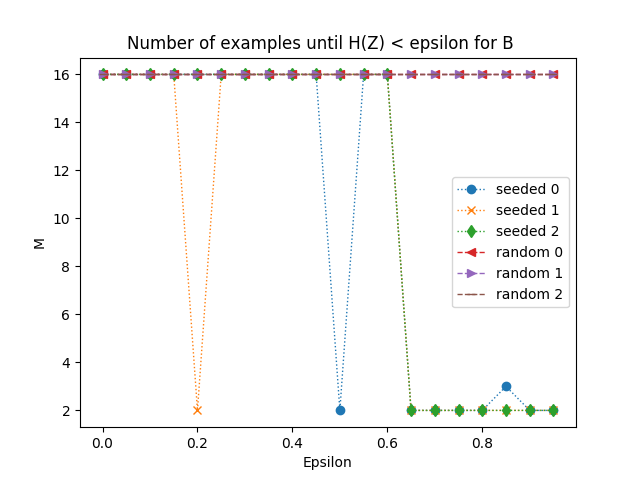
\includegraphics[width=\linewidth]{figs/thm1_allbs.png}
\end{centering}
\caption{\label{fig:thm1}}
\end{figure}

\begin{figure}
\begin{centering}
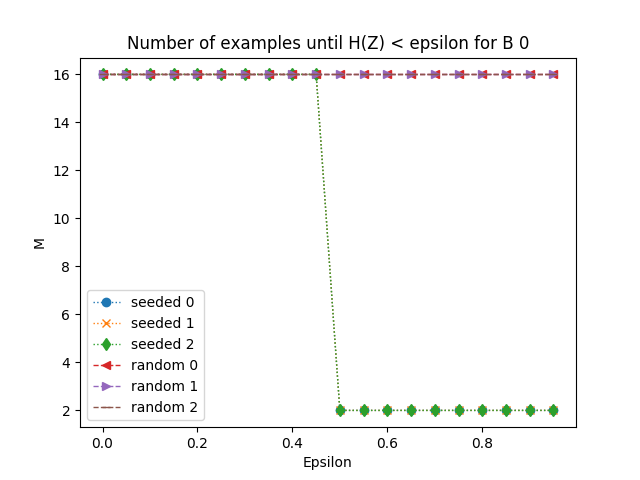
\includegraphics[width=\linewidth]{figs/seeded_0.png}
\end{centering}
\caption{\label{fig:b0}}
\end{figure}

\begin{figure}
\begin{centering}
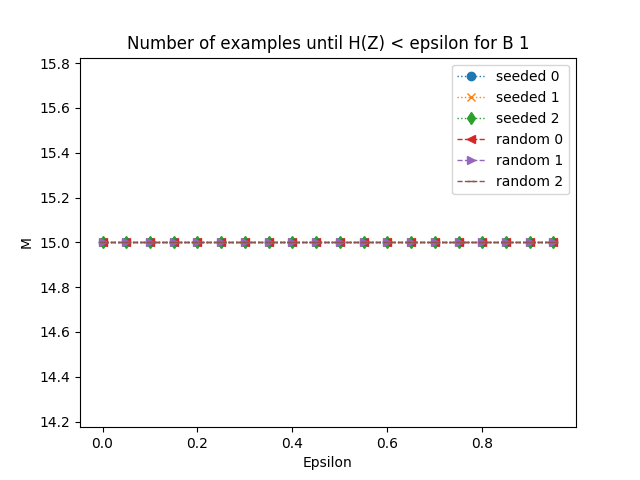
\includegraphics[width=\linewidth]{figs/seeded_1.png}
\end{centering}
\caption{\label{fig:b1}}
\end{figure}

\begin{figure}
\begin{centering}
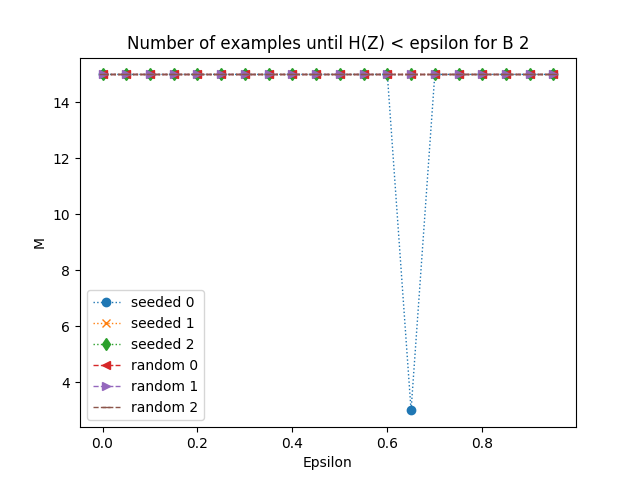
\includegraphics[width=\linewidth]{figs/seeded_2.png}
\end{centering}
\caption{\label{fig:b2}}
\end{figure}

\begin{figure}
\begin{centering}
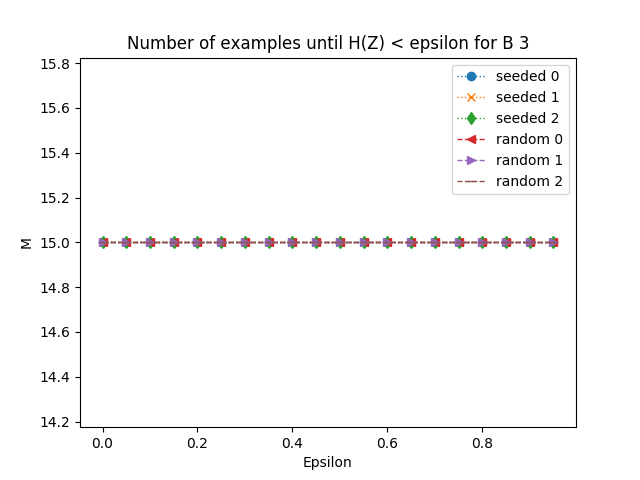
\includegraphics[width=\linewidth]{figs/seeded_3.png}
\end{centering}
\caption{\label{fig:b3}}
\end{figure}

\begin{figure}
\begin{centering}
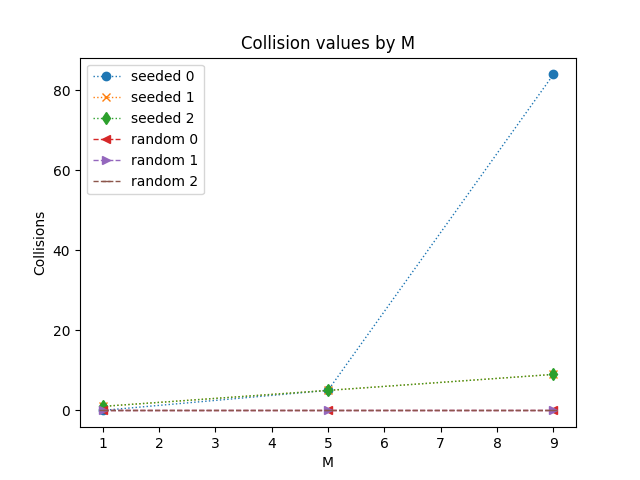
\includegraphics[width=\linewidth]{figs/collisions_0.png}
\end{centering}
\caption{\label{fig:col0}}
\end{figure}

\begin{figure}
\begin{centering}
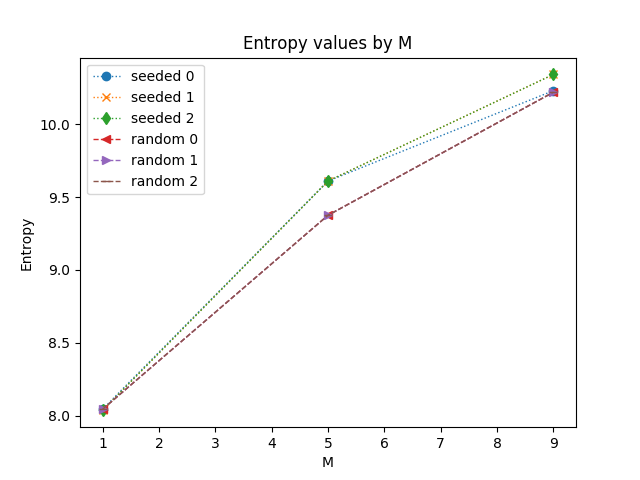
\includegraphics[width=\linewidth]{figs/entropy_0.png}
\end{centering}
\caption{\label{fig:ent0}}
\end{figure}

\begin{enumerate}
\item Seed sampling algorithm with known collisions and see if other collisions are uncovered. Logic is based on the fact that tunneling properties provide necessary but not sufficient conditions for collisions 
\item Can test with SHA1 as well
\item Run the sampling scheme for different values of $\epsilon, \delta$ and see the collision rates, yields of $\hat{X}$
\item Derive $m$ for Theorem 1 given different values of $\epsilon, \delta$ and map that to reasonable CPU measures. Then test this empirically and validate our values of $\epsilon, \delta$ measure up empirically (Frame in terms of threat model) 
\item Run on known good hash functions (ie SHA256) and see what results we get
\end{enumerate}

\textbf{Figure out:} What charts do we want to show? How do we want to structure the results section in the most effective way possible? Options are: 

\begin{enumerate}
\item Table of $m, \epsilon, \delta$, CPU measures for naive algorithm, Theorem 2 alg, alg for uncovering each weakness
\item A chart of CPU/cores vs time it took to run
\item Can have bar charts that illustrate how many times (over N runs), we found a collision, etc
\item Replicate these for the case where we seed the sampling algorithm with known collisions
\end{enumerate}

%-------------------------------------------------------------------------------
\section{Future Work}
%-------------------------------------------------------------------------------

There are three types of work to be pursued following this paper. These directions are, respectively, (1) exploring other types of weaknesses, (2) applying the methodology to other hash functions, and (3) running the presented algorithms on a larger state space. Each of these directions will be taken up in turn in this section. 
\\
\\
First, additional algorithms can be developed to leverage the framework presented in this paper towards discovering other types of weaknesses in hash functions. In addition to being collision resistant, cryptographic hash functions should be resistant to preimage and correlation attacks. The notion of discovering states that are susceptible to collisions can be used to reduce the work load on a SAT solver attempting a preimage attack by reducing the amount of unknown intermediate states. SAT solvers have been successfully applied to hash functions in similar contexts ~\cite{mironov2006applications}. Additional algorithms could be developed for correlation attacks. 
\\
\\
Secondly, this methodology should be applied to other hash functions. One of the key strengths of our framework is that it can easily be applied to any hash function of the Merkle{\textendash}Damg\r{a}rd construction. In this paper we explored applications to MD5, but more computationally expensive applications of the framework should be carried out against SHA1 and SHA2 in pursuit of winding weaknesses of these hash functions. 
\\
\\
Lastly, greater computational resources can be applied to find additional interesting properties of MD5. Due to resource constraints, we could only apply our framework to explore an input space of  $\sim 2^{21}$. Running the experiments run in this paper on larger input spaces would yield additional interesting results about MD5. 

%-------------------------------------------------------------------------------
\section*{Acknowledgments}
%-------------------------------------------------------------------------------

The USENIX latex style is old and very tired, which is why
there's no \textbackslash{}acks command for you to use when
acknowledging. Sorry.

%-------------------------------------------------------------------------------
\section*{Availability}
%-------------------------------------------------------------------------------

USENIX program committees give extra points to submissions that are
backed by artifacts that are publicly available. If you made your code
or data available, it's worth mentioning this fact in a dedicated
section.

%-------------------------------------------------------------------------------
\section*{Appendix}
%-------------------------------------------------------------------------------
\subsection{Proof of Theorem 1}
We restate Theorem 1 and prove it below:

\begin{theorem}
\label{mainThm}
For a given $\epsilon, \delta$ how many samples $m$, where $m = F(\epsilon, \delta)$ are needed such that $P(\frac{P(Z)}{P_{ideal}(Z)}< \epsilon) > 1 - \delta$ for the state space $Z$ where the set of states are defined in our Markov model. 
\end{theorem}

The proof is as follows:
\\
\\
Chernoff bounds state that if $X$ is a random variable, then for any $a \in R$, $P(X \geq a) = P(e^{sx} \geq e^{sa})$ for $s > 0$. 
\\
\\
By Markov's inequality, we can write $P(X \geq a)  = P(e^{sx} \geq e^{sa}) \leq \frac{E[e^{sx}]}{e^{sa}}$. 
\\
\\
Note that $E[e^{sx}]$ is the moment generating function $M_{x}(s)$. 
\\
\\
$\rightarrow P(X \geq a) \leq e^{-sa} M_{x}(s) \forall s > 0$
\\
\\
$\rightarrow P(X \geq a) \leq $min$_{s >0}$ $e^{-sa} M_{x}(s)$.
\\
\\
$\rightarrow P(H(Z) > C \cdot \epsilon) \leq $min$_{s >0}$ $e^{-sa} M_{x}(s)$.
\\
\\
\textcolor{red}{Write the moment generating function as a function of $m$ and $\delta$}

%-------------------------------------------------------------------------------
\bibliographystyle{plain}
\bibliography{\jobname}

%%%%%%%%%%%%%%%%%%%%%%%%%%%%%%%%%%%%%%%%%%%%%%%%%%%%%%%%%%%%%%%%%%%%%%%%%%%%%%%%
\end{document}
%%%%%%%%%%%%%%%%%%%%%%%%%%%%%%%%%%%%%%%%%%%%%%%%%%%%%%%%%%%%%%%%%%%%%%%%%%%%%%%%

%%  LocalWords:  endnotes includegraphics fread ptr nobj noindent
%%  LocalWords:  pdflatex acks